\chapter{Simulations}


\section{Computational Domain}
\subsection{AMR and Discretization}
Our target simulation is a 3D LES with a grid size that is 100 times larger than the smallest scale of the turbulent flow. This smallest scale of these turbulent flows, known as the Kolmogorov scale \cite{kolmogorov}, can be approximated as:
\begin{equation} \label{Kolmogorov}
	\eta = \left( \dfrac{\nu^3}{\varepsilon} \right)^{1/4}
\end{equation}
where $\nu = \nicefrac{\mu}{\rho}$ is the kinematic viscosity and $\varepsilon = \nicefrac{v_{in}^3}{d}$ is used to approximate the average rate of dissipation of turbulence kinetic energy per unit mass, where $v_{in}$ is the reference inflow velocity in the axial direction $y$ and $d=\SI{.01}{cm}$ is the jet diameter. For these turbulent jets, $\eta = \SI{5.37e-6}{cm}$. In our setup, the domain length in each direction is $x = 25d$, $y = 62.5d$, and $z = 25d$. To keep the calculation tractable \cite{} and achieve an adequate \gls{les} grid size, we implement four levels of refinement, with a refinement ratio of 2, leading to 80, 200, and 80 cells on the coarsest level in the $x$, $y$, and $z$ directions, respectively. This results in an initial mesh size of $\Delta x_{0}=\Delta y_{0}=\Delta z_{0}=0.3125$, leading to $\Delta x_{3}=\Delta y_{3}=\Delta z_{3}=\SI{3.9062e-4}{}$, where the subscript denotes the \gls{amr} level. The full four levels of refinement are implemented in a box around the inlet of lengths $x=z=4d$ and $y=2d$ to ensure high refinement at the inflow. These four levels are then adaptively refined based on the given refinement criterion in the region outward from the jet inlet up to a distance of $20d$ in the $x$ and $z$ direction and $60d$ in the $y$ direction, as can be seen in Figure \ref{fig:domain}. The refinement criterion is given by the vorticity, specifically with $\omega \geq 5000^{2l}$, where $\omega$ is the magnitude of the vorticity and $l$ is the \gls{amr} level. For the first ten flow throughs of the simulation, mesh refinement only occurs up to one level within the refinement region to establish the flow pattern. Thereafter, the simulation proceeds with the four levels of mesh refinement for ten more flow-throughs. After that, statistics are collected over the next two flow-throughs for analysis, where a steady state is assumed to have been reached.
\begin{figure}[h!]
\centering
\begin{tikzpicture} [scale = .6]
	\draw [draw=c3med, fill=c3med!60, thick] (.5, 0) -- (4.5,0) -- (4.5, 12) -- (.5, 12) -- (.5, 0); 
	\draw [draw=c2med, fill=c2med!60, thick] (2.1, 0) -- (2.1, .4) -- (2.9, .4) -- (2.9, 0) -- (2.1, 0); 
	\draw [thick] (0,0) -- (5,0) -- (5,12.5) -- (0,12.5) -- (0,0);
	\draw [ultra thick] (2.4,0) -- (2.6, 0);
	\node [below] at (2.6,0) {\scriptsize{Jet Inlet}};
	\node [below] at (2.6,-.5) {\scriptsize{$v_{in}$, $T_{in}$}};
	\node [right] at (0.8, 10.4) {\scriptsize{Ambient Fluid}};
	\node [right] at (1.6, 9.9) {\scriptsize{$v_{\infty} = 0$}};
	\node [right] at (1.6, 9.4) {\scriptsize{$T_{\infty}$, $p_{\infty}$}};
	\node [right] at (5, 6.25) {\footnotesize{$62.5d$}};
	\node [above] at (2.5, 12.5) {\footnotesize{$25d$}};
	%\node [below, c2med] at (.8, 2.2) {\tiny{4 levels}};
	%\node [below, c3med] at (6.25, .6) {\tiny{$\omega$ refinement}};
	\node [below] at (2.5, 12.6) {\scriptsize{Outflow BC}};
\end{tikzpicture}
\hspace{.1in}
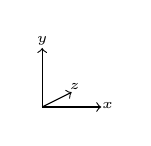
\begin{tikzpicture} [scale = .75]
	\draw [<->] (0,2.15) -- (0,1.15) -- (1,1.15);
	\draw[->] (0,1.15) -- (.5,1.4);
	\node [right] at (.85,1.175) {\tiny{$x$}};
	\node [right] at (.3, 1.5) {\tiny{$z$}};
	\node [above] at (0,2.025) {\tiny{$y$}};
\end{tikzpicture}
\caption{Two dimensional slice schematic of jet setup. Four levels of refinement are enforced within the green box based on proximity to jet inlet. Refinement based on vorticity criterion then occurs within the blue region. Outside the blue region, \gls{amr} is explicitly turned off to allow flow structures to be dissipated numerically and allowed to leave the domain without incurring spurious reflections.}
\label{fig:domain}
\end{figure}

\subsection{Initial and Boundary Conditions}
Our inlet consists of an opening centered in the $xz$-plane with diameter $d=\SI{.01}{cm}$ through which the \gls{sco2} jet is initialized. The pressure in the jet at the inlet is the same as that of the quiescent background fluid and it is given by $p_{in}=p_{\infty}=\SI{1.01325e+8}{Bayre}$. The ambient fluid remains at rest while the jet is initialized with an inflow velocity of $v_{ref} = \SI{1800}{cm.s^{-1}}$, leading to a Reynolds number of the initialized jet of $Re_{ref} = 22910$, with $v_{ref}$ and $d$ being the reference velocity and length scale respectively. For the jet temperature and pressure conditions given, the inflow density is $\rho_{in}=$ \SI{3.019e-1}{g.cm^{-3}}, as calculated via the \gls{srk} in \textit{PeleC}. To implement a turbulent inflow, we formulate our mean velocity and \gls{rms} values by scaling, interpolating, and adding noise to a predetermined velocity profile calculated via \gls{dns} \cite{DNS}, with jet diameter $D$, axial velocity $v_{\text{\tiny{DNS}}}$, and \gls{rms} values given by $v^{\prime}_{\text{\tiny{DNS}}} =  \langle v_{\text{\tiny{DNS}}}^2 \rangle ^{1/2}$. For \gls{dns} quantities, $(u,v,w)$ values are in the $(r,v,\theta)$ direction. Finalized values are converted to Cartesian values for the simulation. We begin by scaling the \gls{dns} values with our reference jet velocity and length values:
\begin{subequations} \label{Jet_Inflow}
	\begin{align}
		r_{\text{\tiny{DNS}},\ scaled} &= d \cdot \left( \dfrac{r}{D} \right)_{\text{\tiny{DNS}}} \\
		v_{\text{\tiny{DNS}},\ scaled} &=  v_{ref} \cdot v_{\text{\tiny{DNS}}} \\
		v^{\prime}_{\text{\tiny{DNS}},\ scaled} &=  v_{ref} \cdot v^{\prime}_{\text{\tiny{DNS}}} \\
		u^{\prime}_{\text{\tiny{DNS}},\ scaled} &=   v_{ref} \cdot u^{\prime}_{\text{\tiny{DNS}}} \\
		w^{\prime}_{\text{\tiny{DNS}},\ scaled} &=   v_{ref} \cdot w^{\prime}_{\text{\tiny{DNS}}} 
	\end{align}
\end{subequations}  
These values are then linearly interpolated onto our grid values $r(i)$ with $f_1 = \tfrac{r(i) - r_{\text{\tiny{DNS}},\ scaled}(i) }{r_{\text{\tiny{DNS}},\ scaled}(i+1) - r_{\text{\tiny{DNS}},\ scaled}(i)}$, $f_2 = \tfrac{r(i) - r_{\text{\tiny{DNS}},\ scaled}(i+1) }{r_{\text{\tiny{DNS}},\ scaled}(i) - r_{\text{\tiny{DNS}},\ scaled}(i+1)}$, and $\phi_{\text{\tiny{DNS}},\ inter} = f_1\ \phi(i) + f_2\ \phi(i+1)$, where $\phi$ is each of the velocity components mentioned in Equations \ref{Jet_Inflow}. Finally, noise is added to each cylindrical component of the velocity as follows before conversion back to Cartesian coordinates for use in the boundary inflow:
\begin{subequations} \label{Jet_Inflow_noise}
	\begin{align}
		v_{in,\ cyl} &= \langle v_{\text{\tiny{DNS}},\ inter} \rangle + \big(  v^{\prime}_{\text{\tiny{DNS}}, inter}  + \beta  v^{\prime}_{\text{\tiny{DNS}}, inter}    	\psi_1\sin{\theta_1}  \big) \cdot \psi_2 \sin{\theta_2} \label{y_flow} \\
		u_{in,\ cyl} &=   u^{\prime}_{\text{\tiny{DNS}}, inter}  + \beta  u^{\prime}_{\text{\tiny{DNS}}, inter}  \psi_3\sin{\theta_3} \label{t_flow} \\
		w_{in,\ cyl} &=   w^{\prime}_{\text{\tiny{DNS}}, inter}  + \beta  w^{\prime}_{\text{\tiny{DNS}}, inter}  \psi_4\sin{\theta_4}  \label{theta_flow}
	\end{align}
\end{subequations}  
where $\beta = 0.1$ and each $\psi_i$ and $\theta_k$ value is randomly generated as follows:
\begin{subequations} \label{Random_Variables}
	\begin{align}
		r_i &= \sqrt{-2.0 \log{(X_i)}} \label{Random_r} \\
		\theta_k &= 2 \pi X_k \label{Radom_theta}
	\end{align}
\end{subequations}
where $X_n$ are random numbers between 0 and 1. The inflow parameters are finalized as $\phi_{in}$ after being converted to Cartesian coordinates $(r,y,\theta) \to (x,y,z)$. 

We implement zero gradient boundary conditions for all boundaries not involving the jet inflow with first order extrapolations. Additionally, \gls{amr} is halted at a distance of $2.5d$ from the boundary in the $x$ and $z$ directions, and that of $5d$ in the axial direction. This low refinement perimeter is implemented to act in a similar fashion to a sponge with the goal of dissipating waves and thus reducing the chance of spurious reflections from the boundaries.

\section{Case Descriptions}
Three cases are investigated in this study. The first case pertains to an isothermal jet, in which the jet conditions match that of the ambient fluid for all quantities aside from velocity. The other two cases consider non-isothermal jets, in which the ambient fluid is adjusted to no longer match the temperature of the jet inflow. All three cases consider the same inflow conditions, while ambient fluid conditions are what varies between them. Temperatures for the ambient fluid in the non-isothermal cases are chosen such that the ambient fluid is supercritical but the temperature for each case falls on either side of the peak in specific heat seen near the critical point. This peak is associated with the pseudo-boiling phenomenon seen in supercritical fluids, where upon crossing the Widom line, the supercritical fluid experiences a shift from being more gas-like to more liquid-like in nature, although distinct phase separation between the two is not present. A summary of the conditions for each case can be seen in Table \ref{Case-Params}.
\begin{table}[H]
\caption{Summary of jet parameters for each case.}
\label{Case-Params}
\begin{center}
\begin{tabular}{ r || r r r  }
Parameter &Case 1 & Case 2 & Case 3 \\
\hline
$T_{\infty}$ (K)& 330& 350 & 314  \\
$T_{in}$ (K)& 330 & 330 & 330 \\
$p_{\infty}$ (Bayre)& \num{1.01325e+08} & \num{1.01325e+08} & \num{1.01325e+08} \\
$p_{in}$ (Bayre) & \num{1.01325e+08} & \num{1.01325e+08} & \num{1.01325e+08} \\
$\rho_{\infty}$ (g/cm$^3$)& \num{3.0192e-01} & \num{2.2567e-01} & \num{5.1274e-01} \\
$\rho_{in}$ (g/cm$^3$) & \num{3.0192e-01} &\num{3.0192e-01}  & \num{3.0192e-01}  \\
$c_{p_{\infty}}$ (Erg/g*K) &\num{3.389e+07} & \num{1.927e+07} & \num{5.703e+07} \\
$c_{p_{in}}$ (Erg/g*K) & \num{3.389e+07} & \num{3.389e+07} & \num{3.389e+07} \\
$C_{s_{\infty}}$ (cm/s) & \num{2.593e+04} & \num{2.661e+04} & \num{3.131e+04} \\
$C_{s_{in}}$ (cm/s) & \num{2.593e+04} & \num{2.593e+04}&\num{2.593e+04} \\
$\mu_{\infty}$ (P) & \num{2.748e-04} & \num{2.445e-04} & \num{4.110e-04} \\
$\mu_{in}$ (P) & \num{2.748e-04} & \num{2.748e-04} & \num{2.748e-04} \\
$\lambda_{\infty}$ (Erg/(cm*s*K))  & \num{3.966e+03}  & \num{3.443e+03} & \num{6.361e+03}  \\
$\lambda_{in}$ (Erg/(cm*s*K))  & \num{3.966e+03} & \num{3.966e+03} & \num{3.966e+03} \\
$Z_{\infty}$ & \num{5.329e-01} & \num{6.691e-01} & \num{3.331e-01} \\
$Z_{in}$ & \num{5.329e-01}& \num{5.329e-01}& \num{5.329e-01}\\
$v_{ref}$ (cm/s)& 1800 & 1800 & 1800  \\
$R_{ref}$ & 22911 & 22911 & 22911  \\
$M_{ref}$ & 0.08 & 0.08 & 0.08  \\

\end{tabular}
\end{center}
\end{table}

The goal in choosing the ambient temperature in this way is to investigate the impact of large thermodynamic changes on the flow field of the supercritical jet. An example of this can be seen with the sharp peak in constant pressure specific heat in Figure \ref{cp_vs_case}. This choice differs from similar studies, which typically involve transcritical injection. 

\begin{figure}[H]
\begin{center}
\includegraphics[scale=0.75]{figures/Plots/NIST/cp_cases.pdf}
\end{center}
\caption{Extreme thermodynamic variation seen near critical point with ambient temperatures plotted for reference to see regime coverage of each case. Red is the jet temperature for all cases and isothermal temperature for the ambient case. Blue is the $350 K$ ambient case. Green is the $314 K$ ambient case. }
\label{cp_vs_case}
\end{figure}

\section{Compute Time and Hardware Specifications}
Simulations were run on the \gls{nrel} Eagle supercomputer using the Intel suite of compilers. Simulations utilized 576 MPI ranks in total, with 36 ranks spread across 16 nodes. Roughly 17,000 cells were handled per MPI rank. Dynamic load balancing of AMR levels allowed for maximum utilization of the system. In total, over 100 TB of data were stored from the original 3D simulations run over the course of the 10 flow-throughs of the domain needed for averaging procedures. To help manage data storage issues, slicing procedures were implemented to reduce full 3D simulation data down to 2D slice data, where averaging procedures were then performed as outlined in the next section. 
\section{Post-Processing Procedures}
Post-processing procedures were written in Python and primarily leveraged the following libraries: yt, pandas, numpy, and, matplotlib. Original 3D data at each plotfile was sliced in three different ways using yt: along the centerline to create 1D data, normal to the jet axis at various points down stream to create 2D data, and along the axial direction at $z=0$ to create 2D data. 

For time averaging, a basic discrete averaging procedure was implemented over $i$ saved plot files from the final 2 flow-throughs of the simulation, with 100 plots saved per flow-through:
\begin{equation} \label{discrete_time_avg}
\phi_{avg,\ slice} = \dfrac{1}{200} \sum\limits_{i=1}^{200} \phi_{i,\ slice}
\end{equation}
For each slice normal to the jet axis, radial averages are approximated with $r = 0$ lying in the center of the $xz-$plane with $r = \sqrt{x^2 + z^2}$. The $N$ points nearest to each fixed $r$ distance away from the center were then averaged together:
\begin{equation} \label{discrete_time_avg}
\phi_{avg,\ r} = \dfrac{1}{N} \sum\limits_{k=1}^{N} \phi_{k,\ r}
\end{equation}
For quantities that were averaged both temporally and radially, temporal averaging was performed first, with the radial average then taken of the time averaged slice data. Fluctuating quantities are calculated on 2D slices via the formulation in Equation \ref{rey_decomp}, with Equation \ref{discrete_time_avg} serving as the approximation for the Reynolds average:
\begin{equation} \label{discrete_rey_decomp}
\phi'_{i,\ slice} = \phi_{avg,\ slice} - \phi_{i,\ slice}
\end{equation}
These perturbations can then be used to calculate average resolved Reynolds stresses for each $u_i$ component of velocity, $\langle u'_i u'_j \rangle$, and \gls{tke} components \cite{iso_comp_2} as follows: 
\begin{equation} \label{TKE}
\langle TKE \rangle = \dfrac{1}{2} \left( \langle u' u' \rangle + \langle v' v' \rangle + \langle w' w' \rangle  \right)
\end{equation}
In Chapter 5, when these quantities are introduced, they are presented without angle brackets for the sake of streamlining bulky notation, but note that all of the results presented from here on are averaged either temporally or temporally and radially as was presented in this section, unless explicitly stated otherwise. 

\section{Challenges and Lessons Learned}
Early challenges in this project were related to the inflow and outflow boundary conditions. We initially compared a few different jet inflow strategies, namely one involving parabolic pipe flow, a \gls{dns} interpolation scheme with added synthetic perturbation \cite{}, and a hyperbolic tangent profile with the same added synthetic perturbation. The interpolation scheme was ultimately selected as it was based on a realistic, pre-developed turbulent pipe flow \cite{} as opposed to being modeled as in the other two cases. This inflow also achieved a fully developed turbulent flow faster than the other two again due to the fact that it was initialized from a pre-developed turbulent flow. Outflow boundary conditions were more complicated. Initially, no \gls{amr} cutoff was implemented at the boundary. After many test runs of varying length (some taking as long as 3 days) where \gls{nscbc} were implemented \cite{} with various mesh sizes, we were still getting non-negligible back flow at the outlet of the domain due to remaining high vorticity levels. Comparisons of mesh size effect on the outflow back flow then led to the buffer zone implementation idea. Various buffer sizes were tested to ensure adequate damping of any spurious outflow feedback. This process alone was a considerable portion of the ten week internship that started this project, before any \gls{les} were even performed. To summarize, during this time, I directly contributed to and tested a variety of Fortran-based inflow and outflow boundary conditions. This process is what led to the boundary condition choices outlined in the above section.

It then took an additional semester's worth of time to troubleshoot \gls{les}-related issues involving \gls{sgs} models, remote access to \gls{nrel}'s Eagle supercomputer, and memory issues. Tests were run to see how distribution of cores per node affected memory, with runs done using 16 cores distributed evenly across 1, 2, and 4 nodes. More nodes also meant longer queue times in the Slurm workload manager, so number of nodes selected ultimately had to strike a balance between best memory distribution for job wait time and execution. It is hard to say exactly how long in total the three simulations took. An error in the root finding routine for the \gls{eos} initially slowed things down for a few months (note: simulations were not continually running during this three month period). After that was corrected, but before switching to the Intel suite of compilers, as of March 29, 2020, the three cases were at the following status: the $330 K$ ambient case still needed 176 hours to reach the final target time for 10 flow throughs, while the $350 K$ and $314 K$ ambient cases needed approximately 696 hours and 3,896 hours, respectively. Though introduced very late into the runs, the Intel suite of compilers did greatly reduce the amount of time left to complete the simulations. 

Post-processing issues relating to slicing posed a major challenge. Upon initial slicing of the 3D data for visualization and averaging, we observed vast portions of data missing, as can be seen in Figure \ref{yt_issue}. These missing data chunks affected slices randomly and did not always correspond to the same \gls{amr} level, making the issue difficult to diagnose. Slicing using \textit{VisIt} revealed the data to be intact, leading to the conclusion that the issue was in our in-house Python slicing script. After including this issue in my SIAM CSE 2021 presentation, we were able to collaborate with members of the Center for Computational Sciences and Engineering (CCSE) group at Lawrence Berkeley National Laboratory. Through this interaction, Andrew Myers of CCSE found a floating point precision bug in yt that was causing the slicing issue. Through this collaboration, yt was improved and we were able to continue with our slicing and data acquisition. 

\begin{figure}[H]
\begin{center}
\includegraphics[scale=0.75]{figures/yt_issue.pdf}
\end{center}
\caption{An example of the yt slicing issue caused by a floating point precision error. The image contains a slice normal to the flow axis depicting the axial velocity component with patches of data missing.}
\label{yt_issue}
\end{figure}

Data storage and transfer issues also created a few hurdles that required strategic thinking to overcome. As mentioned earlier, the three cases in total ended up using over 100 terabytes (TB) of storage on NREL's Eagle. Before data analysis could be completed, the project folder housing the data expired, resulting in the need to either move the full 100 TB of data elsewhere or downscale and move what was feasible within the two week window remaining before deletion. We ultimately decided on deleting all but one of the full plot files from each of the flow-throughs. A checkpoint file was also saved for each flow-through. Slices were then made for the last 200 plot files before being moved to a local hard drive via the Globus file transfer system. These slices only contained vital state data, such as density, temperature, pressure, velocity, etc., to optimize space, leaving secondary data that could be re-calculated from the saved quantities using the system models (like viscosity or internal energy, for example). Slice files were saved in compressed numpy format (.npz) to further optimize storage. This process reduced the data down to under 4 TB, which was much easier to manage. 

An unexpected issue then arose when trying to re-compute derived quantities for further analysis. Transport and thermodynamic models are written in C++ within \textit{PelePhysics}, while the state data of the slices was saved with Python formatting. In order to try to reuse the functions in \textit{PelePhysics}, we explored  strategies to convert Python to C++ arrays. This tactic proved unsuccessful. Instead, I wrote a Python script that combined the necessary \textit{PelePhysics} functions and \gls{co2} transport and thermodynamic properties to recalculate the additional quantities of interest needed for flow analysis. This script can be easily modified for other fluids of interest and provides an avenue for data management in the future. 


\section{Contributions Made to \textit{PelePhysics}}
For direct use in this simulation, I helped create the pure \gls{co2} model folder containing all of the appropriate thermodynamic, transport, and chemical information in the CHEMKIN file format \cite{}. Tangentially related to this project, I also heavily contributed to the the implementation of \gls{qssa} within \textit{PelePhysics}. The Python library I helped create takes user specified QSS species for a given compound model and determines the reactions and related species that are needed to formulate the simplified algebraic expressions needed to update these species within the simulation. This process utilizes Tarjan's Simply Connected Component algorithm \cite{} to formulate a species-species and species-reaction network for determining reaction dependencies. Although the simulations in this project specifically don't contain reacting terms, this \gls{qssa} implementation can be used for future work involving \gls{sco2} applications in direct-firing power systems. Since chemistry is typically the stiffest, and consequently most expensive, component of reacting flow simulations, implementing \gls{qssa} into \textit{PelePhysics} has the potential to greatly reduce system run time and computational cost. A paper is currently in preparation regarding this \gls{qssa} implementation within \textit{PelePhysics}.













